\renewcommand{\theequation}{\theenumi}
\begin{enumerate}[label=\arabic*.,ref=\thesubsection.\theenumi]
\numberwithin{equation}{enumi}
	\item A coin is tossed 1000 times with the following frequencies:\\
Head : 455, Tail : 545\\
Compute the probability for each event.\\
\solution
\renewcommand{\theequation}{\theenumi}
\begin{enumerate}[label=\arabic*.,ref=\thesubsubsection.\theenumi]
\numberwithin{equation}{enumi}
\item In the given question,
\\
The sample size = Total number of possibilities(S)=6
\begin{align}
\myvec{1&2&3&4&5&6}
\end{align}
Event size= Odd number =3
\begin{align}
\myvec{1&3&5}
\end{align}
Probability for this event is = $\frac{1}{2}$
\\
The python code for the distribution of data,
\begin{lstlisting}
prob/codes/prob6_b.py
\end{lstlisting}
This shows the diagrametic representation of dice with the live update of probability with the role of dice.
\end{enumerate}

   \item Two coins are tossed simultaneously 500 times, and we get\\
       Two heads : 105 times\\
       One head : 275 times\\
       No head : 120 times\\
Find the probability of occurrence of each of these events.\\
\solution
From the given information, the desired equation is
\begin{align}
\norm{\vec{x}-\myvec{-3\\2}}^2 = 4^2
\\
\implies \vec{x}^T\vec{x}+\myvec{6&-4}\vec{x} -3 &=0
\end{align}
The python code for Fig. \ref{fig:4.1.1_circle} is
\begin{lstlisting}
solutions/1/codes/circle/circle1.py
\end{lstlisting}
\begin{figure}[!ht]
\centering
\includegraphics[width=\columnwidth]{./solutions/1/figs/circle/circle1.eps}
\caption{Circle using python}
\label{fig:4.1.1_circle}
\end{figure}


   \item A die is thrown 1000 times with the frequencies for the outcomes 1, 2, 3, 4, 5 and 6 as given in the following Table \ref{table:prob_exam_3}.
Find the probability of getting each outcome.

\begin{table}[!ht]
\centering
\resizebox{\columnwidth}{!}{
\begin{tabular}{ |c|c|c|c|c|c|c| } 
 \hline
 \textbf{Outcome} &1 &2 &3 &4 &5 &6  \\ 
 \hline
 \textbf{Frequency} &179 &150 &157 &149 &175 &190 \\ 
 \hline
\end{tabular}
}
\caption{}
\label{table:prob_exam_3}
\end{table}
%\\
\solution
Let $X \in \cbrak{i}_{i=1}^{6}$ and $f_i$ be the correspnding frequency.  Then, 
\begin{align}
\pr{X=i} &= \frac{f_i}{1000}
\end{align}
The following code computes the probabilities
\begin{lstlisting}
solutions/1-10/codes/probexm/probexm3.py
\end{lstlisting}
%\begin{figure}[!ht]
%	\centering
%	\includegraphics[width=\columnwidth]{./figures/probexm/probexm3.eps}
%	\caption{probability of outcome of biased dice }
%	\label{fig:bts3}
%	\begin{lstlisting}
%	figs/probexm/probexm3.eps
%	\end{lstlisting}
%\end{figure}


   \item On one page of a telephone directory, there were 200 telephone numbers.
The frequency distribution of their unit place digit (for example, in the number 25828573, the unit place digit is 3) is given in Table \ref{table:prob_exam4}
below

\begin{table}[!ht]
\centering
\resizebox{\columnwidth}{!}{
\begin{tabular}{ |c|c|c|c|c|c|c|c|c|c|c| } 
\hline
 \textbf{Digit} &0 &1 &2 &3 &4 &5 &6 &7 &8 &9 \\ 
 \hline
 \textbf{Frequency} &22 &26 &22 &22 &20 &10 &14 &28 &16 &20 \\ 
 \hline
\end{tabular}
}
\caption{}
\label{table:prob_exam4}
\end{table}
Without looking at the page, the pencil is placed on one of these numbers, i.e., the number is chosen at random. What is the probability that the digit in its unit place is 6?\\
\solution
In general, the complex number $\myvec{a_1\\a_2}$ has the matrix representation
\begin{align}
\label{eq:3.4.1_Complex}
\myvec{a_1\\a_2} &= \myvec{a_1 & -a_2\\ a_2 & a_1}\myvec{1\\0}
\\
&= \vec{T}_a\myvec{1\\0}
\\
\implies \myvec{5\\-3}&=\myvec{5&3\\-3&5}\myvec{1\\0}
\end{align}
Then,
\begin{align}
\myvec{5\\-3}^3 &\triangleq\myvec{5&3\\-3&5}^3\myvec{1\\0}
\\
 &= \myvec{-10&198\\-198&-10} \myvec{1\\0}
\\
&=\myvec{-10\\-198}
\end{align}
The python code for above problem is
\begin{lstlisting}
codes/line/comp.py
\end{lstlisting}

%Let $X \in \cbrak{i}_{i=1}^{6}$ and $f_i$ be the correspnding frequency.  Then, 
\begin{align}
\pr{X=i} &= \frac{f_i}{1000}
\end{align}
and
\begin{align} 
\pr{X=6} &= \frac{14}{200}
\\
&= 0.07
\end{align}
The related code is available in 
\begin{lstlisting}
solutions/1-10/codes/probexm/probexm4.py
\end{lstlisting}
%\begin{figure}[!ht]
%	\centering
%	\includegraphics[width=\columnwidth]{./figures/probexm/probexm4.eps}
%	\caption{bernoulli distribution of no to be 6}
%	\label{fig:bt2}
%	\begin{lstlisting}
%	figs/probexm/probexm4.eps
%	\end{lstlisting}
%\end{figure}

   \item The record of a weather station shows that out of the past 250 consecutive days, its weather forecasts were correct 175 times.\\
   (i) What is the probability that on a given day it was correct?\\
(ii) What is the probability that it was not correct on a given day?\\
\solution
In this table max frequency is 8 and modal class related to it is 3-5.
\\
\begin{align}
l &= 3
\\
h = 2
\\
f_1 &= 8
\\
f_0 &= 7
\\
f_2 &= 2
\\
Mode &= l+\frac{f_1 - f_o}{2f_1 - f_o - f_2}\times h
\\
&= 3+\frac{8 - 7}{2\times 8 - 7- 2}\times 2
\\
&=3.28
\end{align}
Related code is available in 
\begin{lstlisting}
codes/static5.py
\end{lstlisting}

\item A tyre manufacturing company kept a record of the distance covered
before a tyre needed to be replaced. Table \ref{table:prob_exam6}
shows the results of 1000 cases.
\begin{table}[!ht]
\centering
\resizebox{\columnwidth}{!}{
\begin{tabular}{ |c|c|c|c|c| } 
 \hline
 \textbf{Distance(in km)} &$>$ 4000 &4000-9000 &9001-14000 &$<$14000 \\ 
 \hline
 \textbf{Frequency} &20 &210 &325 &445\\ 
 \hline
\end{tabular}
}
\caption{}
\label{table:prob_exam6}
\end{table}
If you buy a tyre of this company, what is the probability that :\\
(i) it will need to be replaced before it has covered 4000 km?\\
(ii) it will last more than 9000 km?\\
(iii) it will need to be replaced after it has covered somewhere between 4000 km and 14000 km?\\
\solution
From the given information,
\begin{enumerate}
\item 
\begin{align}
\pr{X>9000} &= \frac{325 +445}{1000}
\\
&=0.77
\end{align}
\item 
\begin{align}
\pr{4000<X<14000} &= \frac{20+210+325}{1000}
\\
&=0.0.555
\end{align}
\item 
\begin{align}
\pr{X<4000} &= \frac{20}{1000}
\\
&=0.02
\end{align}
Related codes are available in 
\begin{lstlisting}
solutions/1-10/codes/probexm/probexm6.py
\end{lstlisting}
%\begin{figure}[!ht]
%	\centering
%	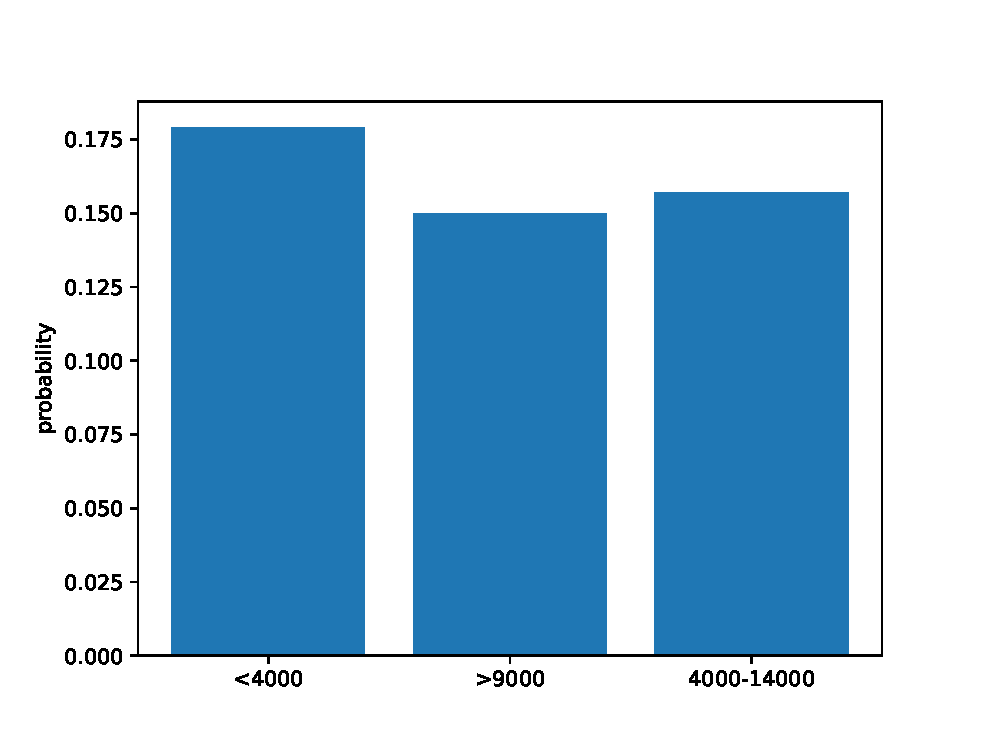
\includegraphics[width=\columnwidth]{./figures/probexm/probexm6.eps}
%	\caption{probability of distance covered by tyre }
%	\label{fig:bt6}
%	\begin{lstlisting}
%	figs/probexm/probexm6.eps
%	\end{lstlisting}
%\end{figure}
\end{enumerate}

\item The percentage of marks obtained by a student in the monthly unit tests are given in Table \ref{table:prob_exam7}
below.
Based on this data, find the probability that the student gets more than 70$\%$ marks in a unit test.\\

\begin{table}[!ht]
\centering
\resizebox{\columnwidth}{!}{
\begin{tabular}{ |c|c|c|c|c|c| } 
 \hline
 \textbf{Unit test} &I &II &III &IV &V \\ 
 \hline
 \textbf{Frequency }&69 &71 &73 &68 &74\\ 
 \hline
\end{tabular}
}
\caption{}
\label{table:prob_exam7}
\end{table}
\solution
From the given information,
\begin{align}
\pr{X>70} &= \frac{3}{5}
\\
&= 0.6
\end{align}


\item An insurance company selected 2000 drivers at random (i.e., without
any preference of one driver over another) in a particular city to find a relationship between age and accidents. The data obtained are given in the Table \ref{table:prob_exam8}.
Find the probabilities of the following events for a driver chosen at random from the city:\\
(i) being 18-29 years of age \textit{and} having exactly 3 accidents in one year.\\
(ii) being 30-50 years of age \textit{and} having one or more accidents in a year.\\
(iii) having no accidents in one year.\\
\begin{table}[!ht]
\centering
\resizebox{\columnwidth}{!}{
\begin{tabular}{|c|c|c|c|c|c|}
\hline
\textbf{Age of drivers} &\multicolumn{5}{c|}{\textbf{Accidents in one year }}\\
\cline{2-6}
(in years) &\textbf{0} &\textbf{1} &\textbf{2} &\textbf{3} &\textbf{over 3}\\
\hline
18-29 &440 &160 &110 &61 &35\\
\hline
30-50 &505 &125 &60 &22 &18\\
\hline
Above 50 &360 &45 &35 &15 &9\\
\hline
\end{tabular}
}
\caption{}
\label{table:prob_exam8}
\end{table}

\solution
Let $X \in {1,2,3}$ represent the random variable representing the age groups of the drivers. Let $Y$ represent the accidents
\begin{enumerate}
\item Then,
\begin{align}
\pr{X=1, Y = 3} &= \frac{61}{2000}
\\
&= 0.03
\end{align}
\item 
\begin{align}
\pr{X=2, Y \ge 1} &= \frac{125+60+22+18}{2000}
\end{align}
\item 
\begin{align}
\pr{Y = 0} &= \frac{440+505+360}{2000}
\\
&= 0.65
\end{align}
Related code is available in 
\begin{lstlisting}
solutions/1-10/codes/probexm/probexm8.py
\end{lstlisting}
%\begin{figure}[!ht]
%\centering
%\includegraphics[width=\columnwidth]{./figures/probexm/probexm8.eps}
%\caption{probability ofaccident in an year }
%\label{fig:bt2}
%\begin{lstlisting}
%figs/probexm/probexm8.eps
%\end{lstlisting}
%\end{figure}
\end{enumerate}


\item Consider the frequency distribution in Table \ref{table:prob_exam9} below which gives the weights of 38 students of a class.
(i) Find the probability that the weight of a student in the class lies in the interval 46-50 kg.\\
(ii) Give two events in this context, one having probability 0 and the other having probability 1.

%
\begin{table}[!ht]
\centering
\resizebox{\columnwidth}{!}{
\begin{tabular}{ |c|c| } 
 \hline
 \textbf{Weights (in kg)} &\textbf{Number of students }\\ 
 \hline
 31-35 &9\\
 36-40 &5\\
 41-45 &14\\
 46-50 &3\\
 51-55 &1\\
 56-60 &2\\
 61-65 &2\\
 66-70 &1\\
 71-75 &1\\
 \hline
 \textbf{Total} &38\\
 \hline
\end{tabular}
}
\caption{}
\end{table}
\solution
\begin{enumerate}
\item 
From the given information, 
\begin{align}
\pr{46<X<50} &= \frac{3}{38}
\\
&= 0.079
\end{align}

\item There is no student whose weight is less than 31 kg thus the probability of a student to have the weight less than 31 kg = 0\\

All of the student in this context  have the weight between 31-75 so we can say that the probability of the students to have the weight in the range 31-75 = 1
\end{enumerate}


\item Fifty seeds were selected at random from each of 5 bags of seeds, and were kept under standardised conditions favourable to germination. After 20 days, the
number of seeds which had germinated in each collection were counted and recorded in Table \ref{table:prob_exam10}

What is the probability of germination of
(i)more than 40 seeds in a bag?\\
(ii) 49 seeds in a bag?\\
(iii) more that 35 seeds in a bag?\\

\begin{table}[!ht]
\centering
\resizebox{\columnwidth}{!}{
\begin{tabular}{ |c|c|c|c|c|c| } 
 \hline
 \textbf{Bag} &1 &2 &3 &4 &5\\ 
 \hline
\textbf{No.of seeds germinated} &40 &48 &42 &39 &41 \\ 
 \hline
\end{tabular}
}
\caption{}
\label{table:prob_exam10}
\end{table}
\solution
Let $X$ represent the seeds and $Y$ represent the bags.
\begin{enumerate}
\item 
\begin{align}
\pr{X > 40} &= \frac{3}{5}
\\
&= 0.6
\end{align}
\item
\begin{align}
\pr{X=49} &= \frac{0}{5}
\\
&= 0
\end{align}
\item 
\begin{align}
\pr{X>35} &= \frac{5}{5}
\\
&= 1
\end{align}
Related code is available in
\begin{lstlisting}
solutions/1-10/codes/probexm/probexm10.py
\end{lstlisting}
%\begin{figure}[!ht]
%	\centering
%	\includegraphics[width=\columnwidth]{./figures/probexm/probexm10.eps}
%	\caption{probability of germinated seeds in a bag }
%	\label{fig:bt10}
%	\begin{lstlisting}
%	figs/probexm/probexm10.eps
%	\end{lstlisting}
%\end{figure}
\end{enumerate}



\item If P(A)=$\frac{7}{13}, P(B)=\frac{9}{13}$ and $P(A\cap B)=\frac{4}{13},$ Evaluate P(A/B)?\\

\item A family has two children. What is the probability that both the children are boys given that at least one of them is a boy?\\

\item Ten cards numbered 1 to 10 are placed in a box, mixed up thoroughly and then one card is drawn randomly. If it is known that the number on the drawn card is more than 3, what is the probability that it is an even number?\\

\item In a school, there are 1000 students, out of which 430 are girls. It is known that out of 430,  10 percentage of the girls study in class XII. What is the probability that a student chosen randomly studies in Class XII given that the chosen student is a girl?\\

\item A die is thrown three times. Events A and B are defined as below:\\
A : 4 on the third throw.\\
B : 6 on the first and 5 on the second throw.\\
Find the probability of A given that B has already occurred?\\

\item A die is thrown twice and the sum of the numbers appearing is observed to be 6. What is the conditional probability that the number 4 has appeared at least once?\\

\item Consider the experiment of tossing a coin. If the coin shows head, toss it again but if it shows tail, then throw a die. Find the conditional probability of the event that "the die shows a number greater than 4" given that "there is at least one tail".\\

\item An urn contains 10 black and 5 white balls. Two balls are drawn from the urn one after the other without replacement. What is the probability that both drawn balls are black?\\

\item Three cards are drawn successively, without replacement from a pack of 52 well shuffled cards. What is the probability that first two cards are kings and the third card drawn is an ace?\\

\item A die is thrown. If E is the event "the number appearing is a multiple of 3" and F be the event "the number appearing is even" then find whether E and F are independent ?\\

\item An unbiased die is thrown twice. Let the event A be "odd number on the first throw" and B the event "odd number on the second throw". Check the independence of the events A and B.\\
\solution
Events A and B are independent.




\item Three coins are tossed simultaneously. Consider the event E "three heads or three tails", F "at least two heads" and G "at most two heads". Of the pairs (E,F), (E,G) and (F,G), which are independent? which are dependent?\\
\solution
Let $X_i \in \cbrak{0,1}$ represent the toss of each coin, with 1 being a head  Let
\begin{align}
X = X_1 + X_2 + X_3
\end{align}
Then, 
\begin{align}
\pr{E} &= \pr{\cbrak{X = 3}+ \cbrak{X = 0} }
\\
&= \pr{X = 3}+ \pr{X = 0} 
\\
&= \comb{3}{3}\brak{\frac{1}{2}}^3+\comb{3}{0}\brak{\frac{1}{2}}^3 
\\
&= \frac{1}{4}
\end{align}
\begin{align}
\pr{F} &= \pr{X \ge 2}
\\
&= \comb{3}{2}\brak{\frac{1}{2}}^3+\comb{3}{3}\brak{\frac{1}{2}}^3 
\\
&= \frac{1}{2}
\end{align}
\begin{align}
\pr{G} &= \pr{X \le 2}
\\
&= 1 - \pr{X > 2}
\\
&=1 - \comb{3}{3}\brak{\frac{1}{2}}^3
\\
&= \frac{7}{8}
\end{align}
Now, 
\begin{align}
\pr{EF} &= \pr{\sbrak{\cbrak{X = 3}+\cbrak{X = 0}}\cbrak{X \ge 2}}
\\
&= \Pr\lbrak{\cbrak{X = 3}\cbrak{X \ge 2}}
\\
&\quad +\rbrak{\cbrak{X = 0}\cbrak{X \ge 2}}
\\
&=\pr{X = 3} = \frac{1}{8}
\label{eq:2122_EF}
\end{align}
Similarly,
\begin{align}
\pr{EG} &= \pr{\sbrak{\cbrak{X = 3}+\cbrak{X = 0}}\cbrak{X \le 2}}
\\
&= \Pr\lbrak{\cbrak{X = 3}\cbrak{X \le 2}}
\\
&\quad +\rbrak{\cbrak{X = 0}\cbrak{X \le 2}}
\\
&=\pr{X = 0} = \frac{1}{8}
\label{eq:2122_EG}
\end{align}
and
\begin{align}
\pr{FG} &= \pr{\cbrak{X \ge 2}\cbrak{X \le 2}}
\\
&= \pr{\cbrak{X = 2}}
\\
&=\comb{3}{2}\brak{\frac{1}{2}}^3 = \frac{3}{8}
\label{eq:2122_FG}
\end{align}
From the above equations we see that
\begin{align}
P\brak{E F} &= P\brak{E}P\brak{F}\\
P\brak{GF} &\neq P\brak{G}P\brak{F}\\
P\brak{E G} &\neq P\brak{E}P\brak{G}
\end{align}
Hence only the pair (E,F) are independent events. The pairs (F,G) and (G,E) are dependent events.

%The sample size = Possible number of tosses=8
%\begin{align}
%\resizebox{\columnwidth}{!}{%
%\myvec{\bmat{HHH}&\bmat{TTT}&\bmat{HHT}&\bmat{HTT}&\bmat{HTH}&\bmat{TTH}\bmat{THT}&\bmat{THH}}
%}
%\end{align}
%Favourable outcome for event E = three Heads (or) three Tails
%\begin{align}
%\myvec{\bmat{HHH}&\bmat{TTT}}
%\end{align}
%
%\begin{align}
%P\brak{E} = \frac{1}{4}
%\end{align}
%
%
%Favourable outcome for event F = atleast two Heads 
%\begin{align}
%\resizebox{\columnwidth}{!}{%
%\myvec{\bmat{HHT}&\bmat{HHH}&\bmat{HTH}&\bmat{THH}}
%}
%\end{align}
%
%\begin{align}
%P\brak{F} = \frac{1}{2}
%\end{align}
%
%Favourable outcome for event G = atmost two Heads
%\begin{align}
%\resizebox{\columnwidth}{!}{%
%\myvec{\bmat{TTT}&\bmat{HHT}&\bmat{HTT}&\bmat{HTH}&\bmat{TTH}\bmat{THT}&\bmat{THH}}
%}
%\end{align}
%
%
%
%\begin{align}
%P\brak{G} = \frac{7}{8}
%\end{align}
%
%
%Favourable outcome for event E$\cap$F
%\begin{align}
%\myvec{\bmat{HHH}}
%\end{align}
%
%\begin{align}
%P\brak{E\cap F} = \frac{1}{8}
%\end{align}
%
%
%Favourable outcome for event F$\cap$G 
%\begin{align}
%\myvec{\bmat{HHH}&\bmat{HTH}&\bmat{THH}}
%\end{align}
%
%\begin{align}
%P\brak{F\cap G} = \frac{3}{8}
%\end{align}
%
%Favourable outcome for event E$\cap$G
%\begin{align}
%\myvec{\bmat{TTT}}
%\end{align}
%
%
%
%\begin{align}
%P\brak{E\cap G} = \frac{1}{8}
%\end{align}
%
%\begin{comment}
%	\begin{lstlisting}
%	/codes/triangle/q2py
%	\end{lstlisting}
%	
%	\begin{figure}[!ht]
%	\centering
%	\includegraphics[width=\columnwidth]{/figs/triangle/q2pdf}
%	\caption{Triangle of Q125}
%	\label{fig:qtwo}	
%	\end{figure}
%	
%
%\end{comment}	
%	
%	
%\end{enumerate}


\item Prove that if E and F are independent events, then so are the events E and $F^{'}$.\\
\solution

	\begin{table}[ht]
    \begin{center}
    	\input{./solutions/20-30/tables/statistics/examples/stat_eg_q3.tex}
  \caption{Marks obtained by students}
   \label{table:statsex_23table1}
   \end{center}	
\end{table}

As we can see from table \ref{table:statsex_23table1}, 9 occurs the maximum number of times.\\
Thus Mode = 9.




\item If A and B are two independent events, then the probability of occurrence of at least one of A and B is given by 1- $P(A^{'}) P(B^{'})$\\
\solution
The following python code computes the median .
	\begin{lstlisting}
	codes/statistics/exercises/q24.py
	\end{lstlisting}
	
	
	\begin{align}
	\text{Median} &= l + \frac{\frac{n}{2} -cf}{f}\times h
	\end{align}
	\begin{align}
	\text{n} = \sum f_{i} = 100 \implies \frac{n}{2} = 50\\
	\end{align}
	$\therefore$ 46-48 is the median class.\\
	Here l is the lower limit of the median class = 46\\
	h is the classinterval =2\\
	cf is the cumulative frequency of the class before median class = 14\\
	f is the frequency of the median class =14

	\begin{align}
	\text{Median} &= 46 + \frac{17.5 - 14}{14}\times 2\\
	\text{Median} &= 46 + 0.5 = 46.5
	\end{align}
	Hence median weight is 46.5
	\begin{table}[ht]
	\begin{center}
    	\input{./solutions/20-30/tables/statistics/exercises/stat_ex_q24_ans.tex}
	\caption{Frequency distribution of the weights of students}
	\label{table:stat_ex_q24_anstable10}
	\end{center}
	\end{table}



\item A person has undertaken a construction job. The probabilities are 0.65 that there will be strike, 0.80 that the construction job will be completed on time if there is no strike, and 0.32 that the construction job will be completed on time if there is a strike. Determine the probability that the construction job will be completed on time.\\
\solution

	 Given the production yield per hectare of wheat of 100 farms of a village. 
		The following python code generates the required ogive.
	\begin{lstlisting}
	./solutions/20-30/codes/statistics/exercises/q25.py
	\end{lstlisting}


	
	\begin{figure}[!ht]
	\centering
	\includegraphics[width=\columnwidth]{./solutions/20-30/figs/statistics/exercises/ex_q25.eps}
	\caption{}
	\label{fig:q25_ogive}	
	\end{figure}
	
	\begin{table}[ht]
	%\begin{center}
    	\input{./solutions/20-30/tables/statistics/exercises/stat_ex_q25_ans.tex}
	\caption{production yield using more than cumulative frequency}
	\label{table:stat_ex_q25anstable4}
	%\end{center}
	\end{table}





\item Bag I contains 3 red and 4 black balls while another Bag II contains 5 red and 6 black balls. One ball is drawn at random from one of the bags and it is found to be red. Find the probability that it was drawn from Bag II.\\
\solution
Let $X \in {1,2}$ represent the Bag  and $Y \in \cbrak{0,1}$ represent the colour, where 1 denotes red.  From the given information,
\begin{align}
\pr{X=1}&=\pr{X=2} = \frac{1}{2}
\\
\pr{Y = 1|X=1} &= \frac{3}{7}
\\
\pr{Y = 1|X=2} &= \frac{5}{11}
\end{align}
Thus,
{\tiny
\begin{align}
\pr{X=2|Y=1} &= \frac{\pr{X=2,Y=1}}{\pr{Y=1}}
\\
&=\frac{\pr{Y=1|X=2}\pr{X=2}}{\pr{Y=1|X=1}\pr{X=1}+\pr{Y=1|X=2}\pr{X=2}}
\\
&=\frac{\frac{5}{11}\times \frac{1}{2}}{\frac{3}{7}\times \frac{1}{2}+\frac{5}{11}\times \frac{1}{2}}
\\
&=\frac{35}{68}
\end{align}
}


\item Given three identical boxes I, II and III, each containing two coins. In box I, both coins are gold coins, in box II, both are silver coins and in the box III, there is one gold and one silver coin. A person chooses a box at random and takes out a coin. If the coin is of gold, what is the probability that the other coin in the box is also of gold?\\
\solution
Let $X \in \cbrak{1,2,3}$ represent the box and $Y_1,Y_2 \in \cbrak{0,1}$ represent the coins, 1 representing gold.  Then,
\begin{align}
\pr{X = 1}&=
\pr{X = 2}=
\pr{X = 3}= \frac{1}{3}
\end{align}
\begin{align}
\pr{Y_1 = 1, Y_2 = 1|X=1} &= 1,
\\
\pr{Y_1 = 1, Y_2 = 1|X=2} &= 0
\end{align}
\begin{multline}
\pr{Y = 1, Y_2 = 0|X=3} 
\\
= \pr{Y_1 = 1, Y_2 = 0|X=3} 
\\
= \frac{1}{2}
\end{multline}
Then
\begin{align}
\pr{Y_1=1|Y_2 = 1} = \frac{\pr{Y_1=1,Y_2=1}}{\pr{Y_2=1}}
\label{eq:2.1.27_prob}
\end{align}
Now,
\begin{multline}
\pr{Y_1=1,Y_2 = 1} 
\\
= \sum_{i}\pr{Y_1=1,Y_2 = 1,X = i}
\\
= \sum_{i}\pr{Y_1=1,Y_2 = 1|X = i}\pr{X = i} = \frac{1}{3}
\label{eq:2.1.27_prob_num}
\end{multline}
and
\begin{multline}
\pr{Y_2 = 1} 
\\
= \pr{Y_1=1,Y_2 = 1}+ \pr{Y_1=0,Y_2 = 1}
\\
= \sum_{i}\pr{Y_1=1,Y_2 = 1|X = i}\pr{X = i} 
\\
\quad + \sum_{i}\pr{Y_1=0,Y_2 = 1|X = i}\pr{X = i} 
\\
= \frac{1}{3}+\frac{1}{6} = \frac{1}{2}
\label{eq:2.1.27_prob_den}
\end{multline}
Substituting from \eqref{eq:2.1.27_prob_num}
and \eqref{eq:2.1.27_prob_den}
in \eqref{eq:2.1.27_prob},
\begin{align}
\pr{Y_1=1|Y_2 = 1} = \frac{\frac{1}{3}}{\frac{1}{2}} = \frac{2}{3}
\label{eq:2.1.27_prob_sol}
\end{align}



\item Suppose that the reliability of a HIV test is specified as follows: Of people having HIV, 90$\%$ of the test detect the disease but 10$\%$ go undetected. Of people free of HIV, 99$\%$ of the test are judged HIV –ve but 1$\%$ are diagnosed as showing HIV +ve. From a large population of which only 0.1$\%$ have HIV, one person is selected at random, given the HIV test, and the pathologist reports him/her as HIV +ve. What is the probability that the person actually has HIV?\\
\solution
Let $X,Y \in \cbrak{0,1}$ represent HIV with 1 being positive.  From the given information,
{\small
\begin{align}
\pr{X = 1|Y=1} &= \frac{9}{10},\pr{X = 0|Y=1} = \frac{1}{10}
\\
\pr{X = 1|Y=0} &= \frac{1}{100},
\pr{X = 0|Y=0} = \frac{99}{100}
\\
\pr{Y=1} &= \frac{1}{1000},
\pr{Y=0} = \frac{999}{1000}
\end{align}
}
Then, 
{\tiny
\begin{multline}
\pr{Y=1|X=1} 
\\
= \frac{\pr{X=1|Y=1}\pr{Y=1}}{\pr{X=1|Y=1}\pr{Y=1}+\pr{X=1|Y=0}\pr{Y=0}}
\\
=\frac{\frac{9}{10}\times \frac{1}{1000}}{\frac{9}{10}\times \frac{1}{1000}+\frac{1}{100}\times \frac{999}{1000}}
=\frac{10}{121}
\end{multline}
}


\item In a factory which manufactures bolts, machines A, B and C manufacture respectively 25$\%$, 35$\%$ and 40$\%$ of the bolts. Of their outputs, 5, 4 and 2 percent are respectively defective bolts. A bolt is drawn at random from the product and is found to be defective. What is the probability that it is manufactured by the machine B?\\
\solution
	  See Table 	\ref{table:stat_ex_q29_quetable6}.
Since the minimum =2 and maximum = 32, we take the intervals as 0-5,5-10 and so on upto 30-35. It can be observed that there are very few engineers whose homes are at more than or equal to 20km distance from their work place and most engineers have their workplace at distance of 0km to 15km from their homes.
	\begin{table}[ht]
	\begin{center}
    	\input{./solutions/20-30/tables/statistics/exercises/stat_ex_q29_que.tex}
	\caption{distance of engineers from their residence to their place of work }
	\label{table:stat_ex_q29_quetable6}
	\end{center}
	\end{table}

	


\item A doctor is to visit a patient. From the past experience, it is known that the probabilities that he will come by train, bus, scooter or by other means of transport are respectively $\frac{3}{10},\frac{1}{5},\frac{1}{10}$ and $\frac{2}{5}.$ The probabilities that he will be late are $\frac{1}{4},\frac{1}{3}$ and $\frac{1}{12},$ if he comes by train, bus and scooter respectively, but if he comes by other means of transport, then he will not be late. When he arrives, he is late. What is the probability that he comes by train?\\
\solution
See Table 	\ref{table:stat_ex_q30_quetable7}
.  Since the minimum =84.9 and maximum = 99.2, we take the intervals as 84-86,86-88 and so on upto 98-100. As the relative humidity is high, the data is about rainy season.\\
\begin{align}
\text{Range} &= \text{Maximum value - Minimum value}\\
\text{Range} &= 99.2 - 84.9\\
\text{Range} &= 14.3
\end{align}

	\begin{table}[ht]
	\begin{center}
    	\input{./solutions/20-30/tables/statistics/exercises/stat_ex_q30_que.tex}
	\caption{Relative humidity in \%}
	\label{table:stat_ex_q30_quetable7}
	\end{center}
	\end{table}


\item A man is known to speak truth 3 out of 4 times. He throws a die and reports that it is a six. Find the probability that it is actually a six.\\

\item A person plays a game of tossing a coin thrice. For each head, he is given Rs 2 by the organiser of the game and for each tail, he has to give Rs 1.50 to the organiser. Let X denote the amount gained or lost by the person. Show that X is a random variable and exhibit it as a function on the sample space of the experiment.\\

\item A bag contains 2 white and 1 red balls. One ball is drawn at random and then put back in the box after noting its colour. The process is repeated again. If X denotes the number of red balls recorded in the two draws, describe X.\\

\item Two cards are drawn successively with replacement from a well shuffled deck of 52 cards. Find the probability distribution of the number of aces.\\

\item Find the probability distribution of number of doublets in three throws of a pair of dice?\\

\item Let X denote the number of hours you study during a randomly selected school day. The probability that X can take the values x, has the following form, where k is some unknown constant.\\
P(X=x)= $\begin{pmatrix} 0.1, if x= 0 \\ kx,if x= 1 or 2 \\ k(5-x), if x= 3 or 4 \\ 0, otherwise \end{pmatrix}$
\begin{enumerate}
\item  Find the value of k.
\item  What is the probability that you study at least two hours ? Exactly two hours? At
most two hours?
\end{enumerate}

\item Let a pair of dice be thrown and the random variable X be the sum of the numbers that appear on the two dice. Find the mean or expectation of X.\\

\item Find the variance of the number obtained on a throw of an unbiased die.\\

\item Two cards are drawn simultaneously (or successively without replacement) from a well shuffled pack of 52 cards. Find the mean, variance and standard deviation of the number of kings.\\

\item Six balls are drawn successively from an urn containing 7 red and 9 black balls. Tell whether or not the trials of drawing balls are Bernoulli trials when after each draw the ball drawn is\\
(i) replaced \\
(ii) not replaced in the urn.\\

\item If a fair coin is tossed 10 times, find the probability of
\begin{enumerate}
\item  exactly six heads
\item  at least six heads
\item  at most six  heads
\end{enumerate}
\solution
In general, the complex number $\myvec{a_1\\a_2}$ has the matrix representation
\begin{align}
\label{eq:3.4.1_Complex}
\myvec{a_1\\a_2} &= \myvec{a_1 & -a_2\\ a_2 & a_1}\myvec{1\\0}
\\
&= \vec{T}_a\myvec{1\\0}
\\
\implies \myvec{5\\-3}&=\myvec{5&3\\-3&5}\myvec{1\\0}
\end{align}
Then,
\begin{align}
\myvec{5\\-3}^3 &\triangleq\myvec{5&3\\-3&5}^3\myvec{1\\0}
\\
 &= \myvec{-10&198\\-198&-10} \myvec{1\\0}
\\
&=\myvec{-10\\-198}
\end{align}
The python code for above problem is
\begin{lstlisting}
codes/line/comp.py
\end{lstlisting}


\item Ten eggs are drawn successively with replacement from a lot containing 10$\%$ defective eggs. Find the probability that there is at least one defective egg.\\
\solution
In general, the complex number $\myvec{a_1\\a_2}$ has the matrix representation
\begin{align}
\label{eq:3.4.1_Complex}
\myvec{a_1\\a_2} &= \myvec{a_1 & -a_2\\ a_2 & a_1}\myvec{1\\0}
\\
&= \vec{T}_a\myvec{1\\0}
\\
\implies \myvec{5\\-3}&=\myvec{5&3\\-3&5}\myvec{1\\0}
\end{align}
Then,
\begin{align}
\myvec{5\\-3}^3 &\triangleq\myvec{5&3\\-3&5}^3\myvec{1\\0}
\\
 &= \myvec{-10&198\\-198&-10} \myvec{1\\0}
\\
&=\myvec{-10\\-198}
\end{align}
The python code for above problem is
\begin{lstlisting}
codes/line/comp.py
\end{lstlisting}


\item Coloured balls are distributed in four boxes as shown in Table \ref{table:1.43_boxes}

\begin{table}[ht!]
\centering
\input{./solutions/20-10/prob/tables/boxes43.tex}
\caption{Distribution of the balls in the boxes}
\label{table:1.43_boxes}
\end{table}
A box is selected at random and then a ball is randomly drawn from the selected box. The colour of the ball is black, what is the probability that ball drawn is from the box III?
\\
\solution
In general, the complex number $\myvec{a_1\\a_2}$ has the matrix representation
\begin{align}
\label{eq:3.4.1_Complex}
\myvec{a_1\\a_2} &= \myvec{a_1 & -a_2\\ a_2 & a_1}\myvec{1\\0}
\\
&= \vec{T}_a\myvec{1\\0}
\\
\implies \myvec{5\\-3}&=\myvec{5&3\\-3&5}\myvec{1\\0}
\end{align}
Then,
\begin{align}
\myvec{5\\-3}^3 &\triangleq\myvec{5&3\\-3&5}^3\myvec{1\\0}
\\
 &= \myvec{-10&198\\-198&-10} \myvec{1\\0}
\\
&=\myvec{-10\\-198}
\end{align}
The python code for above problem is
\begin{lstlisting}
codes/line/comp.py
\end{lstlisting}


\item Find the mean of the Binomial distribution B(4,$\frac{1}{3}$).
\\
\solution
In general, the complex number $\myvec{a_1\\a_2}$ has the matrix representation
\begin{align}
\label{eq:3.4.1_Complex}
\myvec{a_1\\a_2} &= \myvec{a_1 & -a_2\\ a_2 & a_1}\myvec{1\\0}
\\
&= \vec{T}_a\myvec{1\\0}
\\
\implies \myvec{5\\-3}&=\myvec{5&3\\-3&5}\myvec{1\\0}
\end{align}
Then,
\begin{align}
\myvec{5\\-3}^3 &\triangleq\myvec{5&3\\-3&5}^3\myvec{1\\0}
\\
 &= \myvec{-10&198\\-198&-10} \myvec{1\\0}
\\
&=\myvec{-10\\-198}
\end{align}
The python code for above problem is
\begin{lstlisting}
codes/line/comp.py
\end{lstlisting}


\item The probability of a shooter hitting a target is $\frac{3}{4}$. How many minimum
number of times must he/she fire so that the probability of hitting the target at least
once is more than 0.99?
\\
\solution
In general, the complex number $\myvec{a_1\\a_2}$ has the matrix representation
\begin{align}
\label{eq:3.4.1_Complex}
\myvec{a_1\\a_2} &= \myvec{a_1 & -a_2\\ a_2 & a_1}\myvec{1\\0}
\\
&= \vec{T}_a\myvec{1\\0}
\\
\implies \myvec{5\\-3}&=\myvec{5&3\\-3&5}\myvec{1\\0}
\end{align}
Then,
\begin{align}
\myvec{5\\-3}^3 &\triangleq\myvec{5&3\\-3&5}^3\myvec{1\\0}
\\
 &= \myvec{-10&198\\-198&-10} \myvec{1\\0}
\\
&=\myvec{-10\\-198}
\end{align}
The python code for above problem is
\begin{lstlisting}
codes/line/comp.py
\end{lstlisting}


\item {\em: Random Process}A and B throw a die alternatively till one of them gets a '6' and wins the game. Find their respective probabilities of winning, if A starts first.
\\
\solution
In general, the complex number $\myvec{a_1\\a_2}$ has the matrix representation
\begin{align}
\label{eq:3.4.1_Complex}
\myvec{a_1\\a_2} &= \myvec{a_1 & -a_2\\ a_2 & a_1}\myvec{1\\0}
\\
&= \vec{T}_a\myvec{1\\0}
\\
\implies \myvec{5\\-3}&=\myvec{5&3\\-3&5}\myvec{1\\0}
\end{align}
Then,
\begin{align}
\myvec{5\\-3}^3 &\triangleq\myvec{5&3\\-3&5}^3\myvec{1\\0}
\\
 &= \myvec{-10&198\\-198&-10} \myvec{1\\0}
\\
&=\myvec{-10\\-198}
\end{align}
The python code for above problem is
\begin{lstlisting}
codes/line/comp.py
\end{lstlisting}


\item If a machine is correctly set up, it produces 90$\%$ acceptable items. If it is
incorrectly set up, it produces only 40$\%$ acceptable items. Past experience shows that
80$\%$ of the set ups are correctly done. If after a certain set up, the machine produces 2 acceptable items, find the probability that the machine is correctly setup.
\\
\solution
In general, the complex number $\myvec{a_1\\a_2}$ has the matrix representation
\begin{align}
\label{eq:3.4.1_Complex}
\myvec{a_1\\a_2} &= \myvec{a_1 & -a_2\\ a_2 & a_1}\myvec{1\\0}
\\
&= \vec{T}_a\myvec{1\\0}
\\
\implies \myvec{5\\-3}&=\myvec{5&3\\-3&5}\myvec{1\\0}
\end{align}
Then,
\begin{align}
\myvec{5\\-3}^3 &\triangleq\myvec{5&3\\-3&5}^3\myvec{1\\0}
\\
 &= \myvec{-10&198\\-198&-10} \myvec{1\\0}
\\
&=\myvec{-10\\-198}
\end{align}
The python code for above problem is
\begin{lstlisting}
codes/line/comp.py
\end{lstlisting}

\item Find the probability of getting a head when a coin is tossed once. Also
find the probability of getting a tail.
\\
\solution
In general, the complex number $\myvec{a_1\\a_2}$ has the matrix representation
\begin{align}
\label{eq:3.4.1_Complex}
\myvec{a_1\\a_2} &= \myvec{a_1 & -a_2\\ a_2 & a_1}\myvec{1\\0}
\\
&= \vec{T}_a\myvec{1\\0}
\\
\implies \myvec{5\\-3}&=\myvec{5&3\\-3&5}\myvec{1\\0}
\end{align}
Then,
\begin{align}
\myvec{5\\-3}^3 &\triangleq\myvec{5&3\\-3&5}^3\myvec{1\\0}
\\
 &= \myvec{-10&198\\-198&-10} \myvec{1\\0}
\\
&=\myvec{-10\\-198}
\end{align}
The python code for above problem is
\begin{lstlisting}
codes/line/comp.py
\end{lstlisting}

\item A bag contains a red ball, a blue ball and a yellow ball, all the balls being
of the same size.Kritika takes out a ball from the bag without looking into it. What is the probability that she takes out the
(i) yellow ball? \\
(ii) red ball?\\
(iii) blue ball?
\\
\solution
In general, the complex number $\myvec{a_1\\a_2}$ has the matrix representation
\begin{align}
\label{eq:3.4.1_Complex}
\myvec{a_1\\a_2} &= \myvec{a_1 & -a_2\\ a_2 & a_1}\myvec{1\\0}
\\
&= \vec{T}_a\myvec{1\\0}
\\
\implies \myvec{5\\-3}&=\myvec{5&3\\-3&5}\myvec{1\\0}
\end{align}
Then,
\begin{align}
\myvec{5\\-3}^3 &\triangleq\myvec{5&3\\-3&5}^3\myvec{1\\0}
\\
 &= \myvec{-10&198\\-198&-10} \myvec{1\\0}
\\
&=\myvec{-10\\-198}
\end{align}
The python code for above problem is
\begin{lstlisting}
codes/line/comp.py
\end{lstlisting}

\item Suppose we throw a die once. (i) What is the probability of getting a number greater than 4 ? (ii) What is the probability of getting a number less than or
equal to 4 ?
\\
\solution
In general, the complex number $\myvec{a_1\\a_2}$ has the matrix representation
\begin{align}
\label{eq:3.4.1_Complex}
\myvec{a_1\\a_2} &= \myvec{a_1 & -a_2\\ a_2 & a_1}\myvec{1\\0}
\\
&= \vec{T}_a\myvec{1\\0}
\\
\implies \myvec{5\\-3}&=\myvec{5&3\\-3&5}\myvec{1\\0}
\end{align}
Then,
\begin{align}
\myvec{5\\-3}^3 &\triangleq\myvec{5&3\\-3&5}^3\myvec{1\\0}
\\
 &= \myvec{-10&198\\-198&-10} \myvec{1\\0}
\\
&=\myvec{-10\\-198}
\end{align}
The python code for above problem is
\begin{lstlisting}
codes/line/comp.py
\end{lstlisting}

\item One card is drawn from a well-shuffled deck of 52 cards. Calculate the
probability that the card will\\
(i) be an ace,\\
(ii) not be an ace.
\item Two players, Sangeeta and Reshma, play a tennis match. It is known
that the probability of Sangeeta winning the match is 0.62. What is the probability of
Reshma winning the match?
\item Savita and Hamida are friends. What is the probability that both will have \\
(i) different birthdays? \\
(ii) the same birthday? (ignoring a leap year).
\item There are 40 students in Class X of a school of whom 25 are girls and 15 are boys. The class teacher has to select one student as a class representative. She writes the name of each student on a separate card, the cards being identical.Then
she puts cards in a bag and stirs them thoroughly. She then draws one card from the
bag. What is the probability that the name written on the card is the name of\\
(i) a girl?\\
(ii) a boy?
\item  A box contains 3 blue, 2 white, and 4 red marbles. If a marble is drawn
at random from the box, what is the probability that it will be
(i) white? (ii) blue? (iii) red?
\item Harpreet tosses two different coins simultaneously (say, one is of rupee 1
and other of rupee 2). What is the probability that she gets at least one head?
\item In a musical chair game, the person playing the music has been
advised to stop playing the music at any time within 2 minutes after she starts playing.What is the probability that the music will stop within the first half-minute after starting?
\item A missing helicopter is reported to have crashed somewhere in the rectangular region shown in Fig. 15.2. What is the probability that it crashed inside the
lake shown in the figure?
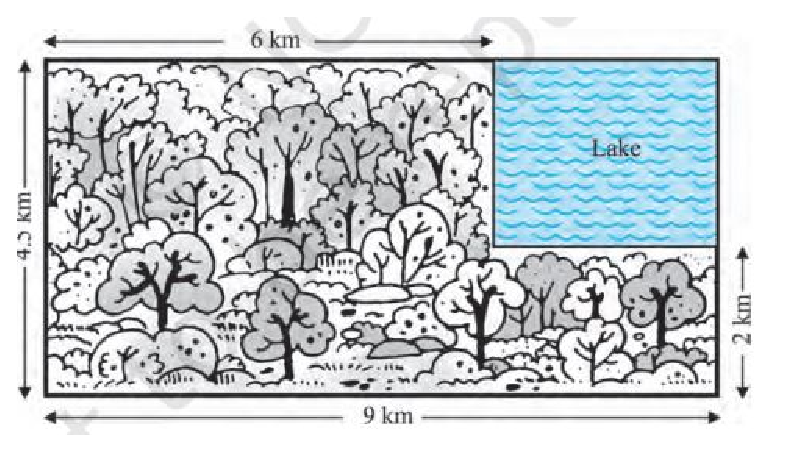
\includegraphics{./prob/figs/lake.eps}\\
\item A carton consists of 100 shirts of which 88 are good, 8 have minor defects and 4 have major defects.Jimmy, a trader, will only accept the shirts which are good, but Sujatha, another trader, will only reject the shirts which have major defects.One shirt is drawn at random from the carton. What is the probability that\\
(i) it is acceptable to Jimmy?\\
(ii) it is acceptable to Sujatha?
\item Two dice, one blue and one grey, are thrown at the same time. Write down all the possible outcomes.What is the probability that the sum of the two numbers appearing on the top of the dice is\\
(i) 8?\\
(ii) 13?\\ 
(iii) less than or equal to 12?\\\\

    \end{enumerate}
%\end{document}
    
